\chapter{Tutorial zu dieser LaTeX-Vorlage}
Dieses Kapitel ist spezifisch für die \LaTeX Vorlage und sollte natürlich in der finalen Abgabe nicht enthalten sein.
Dieser Teil der Arbeit kann bei Bedarf durch einen Kommentar einfach ausgeblendet werden (siehe thesis.tex Zeile 125).






\section{Verwendung dieser Vorlage}
Dieses Template ist für die Verwendung mit pdflatex gedacht. Am einfachsten ist es die Vorlage in Overleaf \cite{overleaf} zu öffnen. Overleaf ist eine Onlineanwendung zum Arbeiten mit \LaTeX{}, was den Vorteil hat, dass nichts lokal installiert werden muss und mit jedem Betriebssystem gearbeitet werden kann, das über einen Browser verfügt. Außerdem ist es möglich mit mehreren Personen gemeinsam an einem Projekt zu arbeiten. Die Vorlage kann auch mit einer lokalen Installation verwendet werden. Die Website von Overleaf bietet zudem einige gute Tutorials zum Arbeiten mit \LaTeX{}: \url{https://www.overleaf.com/learn}.

Fehler und Warnungen, die beim Compilieren erzeugt werden, sollten direkt behoben werden, da es später schwierig sein kann den eigentlichen Auslöser einer Fehlermeldung zu finden. Manchmal sieht das Dokument trotz Fehlermeldung oder Warnung korrekt aus, der Fehler macht sich dann aber später bemerkbar. Die Meldungen sind leider oft nicht sehr aussagekräftig, weshalb es am einfachsten ist direkt nach dem Auftreten eines Fehlers den Teil der Arbeit anzuschauen, der als letztes geändert wurde.

\section{Projektstruktur}

Der Hauptteil einer Thesis besteht üblicherweise aus mehreren Kapiteln, die verschiedene Aspekte der Arbeit beleuchten. 
Es ist ratsam für jedes Kapitel ein eigene Tex-Datei anzulegen, damit der Quellcode übersichtlich bleibt. Durch einen numerischen Präfix (z.B.: \texttt{20\_relatedwork.tex} siehe Abb. \ref{fig:folderstructure}) werden die Quelldateien in der richtigen Reihenfolge in Overleaf angezeigt. Wir verwenden 20 anstatt 2, damit wir nachträglich auch noch 21, 22, etc. einfügen können.

\begin{figure}
    \centering
    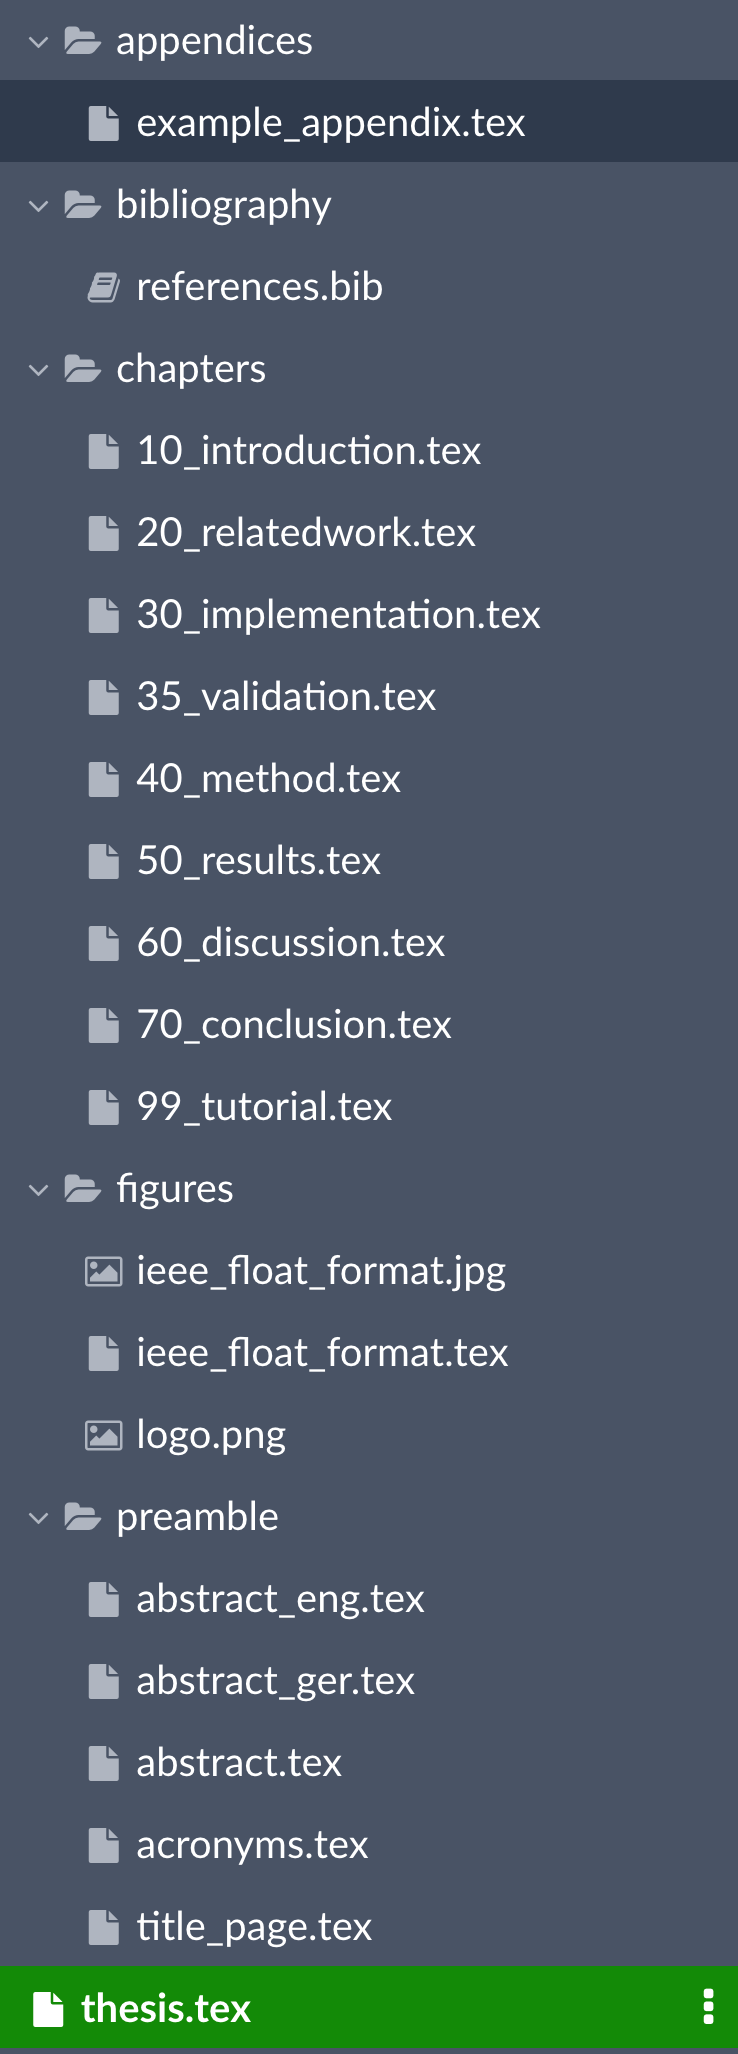
\includegraphics[width=0.4\linewidth]{figures/folderstructure.png}
    \caption{Ordnerstruktur eines LaTeX-Projektes}
    \label{fig:folderstructure}
\end{figure}

\subsection{Unterkapitel}
Unterkapitel sollten ein abgeschlossenes Thema behandeln. Einzelne Unterkapitel in einem Kapitel sind zu vermeiden, also z.\,B. in Kapitel 2 das Unterkapitel 2.1, aber kein weiteres Unterkapitel. In diesem Fall ist es besser entweder den Inhalt von 2.1 direkt in Kapitel 2 zu schreiben, oder falls 2 und 2.1 thematisch zu weit voneinander entfernt sind, aus Unterkapitel 2.1 ein eigenes Kapitel 3 zu machen. Dieses Unterkapitel ist ein negativ Beispiel dafür. 

\section{Grafiken}
In der Informatik sind die häufigsten Grafiken entweder Diagramme oder Plots. Beide Arten von Grafiken lassen sich gut als Vektorgrafiken erstellen und einbinden. Der Vorteil von Vektor- gegenüber Pixelgrafiken ist, dass beliebig weit in eine Grafik hereingezoomt werden kann, ohne dass sie unscharf wird. Zudem benötigen Vektorgrafiken meistens weniger Speicherplatz.

\subsection{Vektor- vs Pixelgrafiken}
Für die meisten Abbildungen sollte man Vektorgrafiken verwenden, diese können verlustfrei skaliert werden und bieten somit die meisten Freiheiten.
Wenn man Grafiken in R erstellt, können die Plots als pdf oder svg-Dateien abgespeichert werden und liegen dann ebenfalls als Vektorgrafik vor. Ein weiteres beliebtes Programm zum Erstellen von Vektorgrafiken ist Inkscape \cite{inkscape}. Zudem bieten viele Programme die Möglichkeit eine Grafik z.\,B. als PDF zu exportieren, was in \LaTeX{} als Vektorgrafik eingebunden werden kann. Adobe Indesign wird auch häufig zum Erstellen von Vektorgrafiken verwendet.

\paragraph{Profi-Tipp TikZ.}
Grafiken können direkt in \LaTeX{} mit dem TikZ Paket \cite{tikz} erstellt werden. Die Verwendung ist etwas gewöhnungsbedürftig, da Grafiken mit Code beschrieben werden, bietet aber viele Freiheiten. Außerdem werden die so erstellten Grafiken direkt in \LaTeX{} gerendert und verwenden die selbe Schriftart wie im Text und eine konsistente Schriftgröße im gesamten Dokument. 

Pixelgrafiken lassen sich nicht immer vermeiden, z.\,B. wenn eine Foto in die Arbeit eingebunden werden soll. In diesem Fall sollte darauf geachtet werden, dass die Grafik über eine ausreichende Auflösung verfügt. Eine Auflösung von 300~dpi ist ein guter Richtwert, um beim Drucken ein gutes Ergebnis zu erhalten.

Abbildungen \ref{fig:ieee_float_format_vector} und \ref{fig:ieee_float_format_pixel} zeigen beide den Aufbau des IEEE Floating Point Formats. Abbidlung \ref{fig:ieee_float_format_pixel} ist eine Pixelgrafik, während Abbildung \ref{fig:ieee_float_format_vector} mit TikZ erstellt wurde. Der Unterschied wird beim hereinzoomen deutlich.

\begin{figure}[ht]
\centering
% Beispiel für eine mit TIKZ erstellte Grafik

\begin{tikzpicture}
[node distance=0cm]
\tikzset{rectangle_black/.style = {rectangle, minimum width=1cm, minimum height=0.75cm, text centered, draw=black, fill=white}};
\tikzset{rectangle_white/.style = {rectangle, minimum width=1cm, minimum height=0.75cm, text centered, draw=none, fill=none}};
\node (sign) [rectangle_black] {S (sign)};
\node (exponent) [rectangle_black, right = of sign] {E (biased exponent)};
\node (fraction) [rectangle_black, right = of exponent] {T (trailing significand field)};
\node (sign_text) [rectangle_white, above = of sign] {1};
\node (exponent_text) [rectangle_white, above = of exponent] {$w$};
\node (fraction_text) [rectangle_white, above = of fraction] {$t=p-1$};
\node (bits) [rectangle_white, above = of fraction, right = of fraction_text] {bits};

\end{tikzpicture}

\caption{Aufbau des IEEE Floating Point Formats als Vektorgrafik mit TikZ erzeugt.}
\label{fig:ieee_float_format_vector}
\end{figure}

\begin{figure}[ht]
\centering
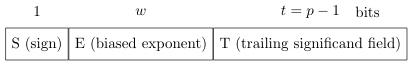
\includegraphics[width=0.65\textwidth]{figures/ieee_float_format.jpg}
\caption{Aufbau des IEEE Floating Point Formats als Pixelgrafik.}
\label{fig:ieee_float_format_pixel}
\end{figure}

\section{Tabellen}
Tabellen können in \LaTeX{} direkt erstellt werden. Tabelle \ref{tab:ieee_formats} zeigt ein Beispiel dafür. Einfache Tabellen lassen sich schnell erstellen, bei komplizierteren Tabellen ist es manchmal einfacher zusätzliche Pakete zu verwenden. Mit dem Paket \texttt{multirow} können z.\,B. einfacher Tabellen erstellt werden, bei denen einzelne Zeilen oder Spalten zusammengefasst sind. 

Unter \url{https://www.tablesgenerator.com/} findet man ein hilfreiches online Werkzeug zum erstellen von Tabellen. Wichtig ist es hier den \textquote{Default table style} zum \textquote{Booktabs table style umzustellen}. 

\begin{table}[ht]
\centering
\begin{tabular}{lrrrr} 
 \toprule
 Parameter & binary16 & binary32 & binary64 & binary128 \\
 \midrule
  $k$, storage width in bits           & 16 &  32 &   64 &   128 \\ 
  $w$, exponent field width in bits    &  5 &   8 &   11 &    15 \\
  $t$, significand field width in bits & 10 &  23 &   52 &   112 \\
  emax, maximum exponent $e$           & 15 & 127 & 1023 & 16383 \\
  bias, $E-e$                          & 15 & 127 & 1023 & 16383 \\
 \bottomrule
\end{tabular}
\caption{IEEE 754-2019 Floating Point Formate als Beispiel für das Einbinden einer Tabelle.}
\label{tab:ieee_formats}
\end{table}

\section{Quellcode}
Um Quellcode in die Arbeit einzubinden, können in \LaTeX{} Listings verwendet werden. Es gibt für populäre Sprachen vorgefertigte Umgebungen, welche die Syntax farblich hervorheben. Quellcode sollte eingebunden werden, wenn eine konkrete Implementierung in einer Sprache erläutert wird. Für die Erklärung eines Algorithmus ist es oft übersichtlicher ein Schaubild oder Pseudocode zu verwenden. Es sollten nur kurze Codeabschnitte eingebunden werden, die für den Leser einfach nachvollziehbar sind und nur den für die Erklärung relevanten Code enthalten. Längere Codeabschnitte können im Anhang stehen. Der komplette Code, der für die Arbeit geschrieben wurde, sollte in einem Repository (Gitlab) % oder Github)
abgelegt werden.

Listing~\ref{lst:example_listing} zeigt ein Beispiel für ein Codelisting in der Programmiersprache C. Algorithmus \ref{alg:west} zeigt einen Routing Algorithmus als Pseudocode. Der Code wurde mit dem Paket algorithm2e \cite{algorithm2e} erstellt.

\begin{lstlisting}[language=C, caption=Beispiel für ein Codelisting in der Sprache C., label=lst:example_listing]
#include <stdio.h>
// comments are highlighted in green
void main() {
    // keywords of the language are highlighted in blue
    for (int i = 0; i <= 42; ++i) {
        printf("%d\n", i);
    }
    // strings are highlighted in red
    printf("Hello World!");
}
\end{lstlisting}

\begin{algorithm}[ht]

    \uIf{destination in west direction}{
        go West;
    }
    \uElseIf{destination in same column}{
        \eIf{destination in north direction}{
            go North;
        }{
            go South;
        }
    }
    \uElseIf{destination in north east direction}{
        go North or go East
    }
    \uElseIf{destination in south east direction}{
        go South or go East
    }
    \uElseIf{destination in same row and in east direction}{
        go East;
    }
    \uElseIf{at destination}{
        done;
}
 \caption{West First-Routing Algorithm.}
 \label{alg:west}
\end{algorithm}

\section{Literatur}
Ein Literaturverzeichnis sollte mit dem apa Paket für BibLatex erstellt werden. Dazu wird für jede Quelle ein Eintrag in der Datei \texttt{references.bib} angelegt. An der passenden Stelle im Text können diese Einträge mit dem \texttt{\textbackslash cite\{\}} Befehl zitiert werden. Für jede Quelle die zitiert wird, legt \LaTeX{}  im Literaturverzeichnis einen Eintrag an.

Beschreibungen der Quellen im Bibtex-Format müssen meistens nicht selbst erstellt werden, sondern können direkt bei vielen Verlagen und Bibliotheken direkt generiert werden. Google bietet mit dem \textquote{Scholar-Button} ein Chromium Plugin, mit dem schnell bibtex-Einträge generiert werden können. Bei Google-Scholar generierten Bibtex-Einträgen muss auch eine manuelle Endkontrolle stattfinden, um zu prüfen, ob die Daten in Google korrekt gespeichert waren (z.B.~fehlende Autoren, falsche Jahreszahl, etc.).

Es gibt verschiedene Arten wie man mit biblatex zitiert.\\
\noindent
\texttt{\textbackslash autocite\{valdez2015reducing\}} führt zu \autocite{valdez2015reducing}.\\
\texttt{\textbackslash parencite\{valdez2015reducing\}} führt zu \parencite{valdez2015reducing}.\\
\texttt{\textbackslash textcite\{valdez2015reducing\}} führt zu \textcite{valdez2015reducing}.\\
\texttt{\textbackslash cite\{valdez2015reducing\}} führt zu \cite{valdez2015reducing}.\\
\texttt{\textbackslash autocite[siehe auch][S. 13]\{valdez2015reducing\}} führt zu \autocite[siehe auch][S.~13]{valdez2015reducing}.\\

Hier\footnote{\url{https://tug.ctan.org/info/biblatex-cheatsheet/biblatex-cheatsheet.pdf}} gibt es ein hilfreiches Cheat-Sheet.

Je nach zitierter Dokumentsorte, sieht die Referenz im Literaturverzeichnis anders aus.
\begin{itemize}
    \item Beispiel für einen Konferenzbeitrag \autocite{Nielsen1990}
    \item Beispiel für einen Journal-Artikel \autocite{hollan2000}
    \item Beispiel für ein Buch~\autocite{zobel2014writing}.
    \item Beispiel für eine Norm~\autocite{ISO9241}.
    \item Beispiel für einen Weblink\footnote{{\url{http://imis.uni-luebeck.de}} \autocite{webimis}}
\end{itemize}

\textbf{Hinweis}: Keine dieser Referenzen müssen Sie in Ihrer Arbeit zitieren!

\section{Abkürzungen}
Für jede verwendete Abkürzung kann ein Eintrag in der Datei \texttt{acronyms.tex} angelegt werden. Wenn diese Abkürzung im Text zum ersten Mal auftaucht, sollte der Begriff ausgeschrieben werden mit der Abkürzung in Klammern dahinter. Bei weiteren Vorkommen im Text kann dann die eigentliche Abkürzung verwendet werden. In \LaTeX{} gibt es dafür spezielle Befehle. Beispiel für ausgeschriebene Abkürzung (siehe Quelltext des Dokuments für die entsprechenden Befehle).

Erste Verwendung mit Erläuterung: \acrfull{nic}.\\ 
Beispiel für das Verwenden der Abkürzung: \acrshort{nic}. 

Die verwendeten Abkürzungen werden automatisch im Abkürzungsverzeichnis aufgelistet.


